 %%LATEX header ********************************************
\documentclass[a4paper, 12pt, titlepage]{article}
\usepackage[utf8]{inputenc}
\usepackage[T1]{fontenc}
\usepackage[danish]{babel}
\usepackage{cite,refstyle,adjustbox,graphicx,amsmath,amssymb,subcaption,varioref,titlesec,comment,amsthm}
\usepackage{mathtools}
\usepackage[dvipsnames]{xcolor}
%\usepackage{epstopdf}
\usepackage{booktabs}
\usepackage{siunitx}
\usepackage{geometry}
\usepackage{setspace}
\usepackage{pgf,tikz,colortbl}
\usepackage{fancyvrb}
\usepackage{floatrow}
\usepackage{parskip}
\DeclareFloatFont{footysize}{\footnotesize}% "scriptsize" is defined by floatrow, "tiny" not
\floatsetup[table]{font=footysize}
%%************************************************************
%%Teorem miljøer 
\newtheorem{antag}{Antagelse}
\newtheorem{teo}{Teorem}
\renewcommand{\arraystretch}{1.3}
%%************************************************************
%%Andet setup
\onehalfspacing
\setlength\heavyrulewidth{0.40ex}
%%************************************************************
%% Makro
\newcommand{\indep}{\perp\!\!\!\perp}
\newcommand{\saa}{\Leftrightarrow}
\newcommand{\pd}[2]{\frac{\partial #1}{\partial #2}}
\newcommand{\Lagr}{\mathcal{L}}
%%************************************************************
%%TIKZ bibliotekter brugt
\usetikzlibrary{shapes,arrows}
% Define block styles
%\tikzstyle{decision} = [diamond, draw, fill=blue!20, text width=4.5em, text badly centered, node distance=3cm, inner sep=0pt]
\tikzstyle{block} = [rectangle, draw, fill=blue!20, 
    text width=8em, text centered, rounded corners, minimum height=4em]
\tikzstyle{line} = [draw, -latex']
\tikzstyle{cloud} = [draw, ellipse,fill=red!20, node distance=3cm,
    minimum height=2em]
%%************************************************************

%%************************************************************
%% Om forfatteren
%%************************************************************
\author{Simon Harmat og Niels Bækgård}
\title{Øvelse i produktivitetspolitik}
\date{\today}
\begin{document}
%\maketitle
%\tableofcontents
\section{Spørgsmål til Asger}
\begin{itemize}
	\item Er der noget galt i at bruge en Cobb Douglas produktionsfunktion til at estimere en eksternalitet?
	\item Produktionsfunktion - translog vs. CF?
	\item Der er helt sikkert et positivt bias i vores model. Er det tilfredsstillende blot at skrive sig ud af det, eller skal der korrieres på en eller anden måde. Bemærk, at vi kun har tilgang til private byerhverv.
	\item Hvad skal vores policy være?
	\begin{itemize}
	 	\item[a.] Planloven: placering af virksomheder, bystørrelsen, 3D-byer ...
	 	\item[b.] Klyngepolitik. Hvilke og hvor store er effekterne af disse?
	 	\item[c.] Government-bashing...
	 	\item[d.] Hvor meget skal artiklen/resume være en opsummering af opgaven? Og hvor meget skal det være et forsøg på at få noget i avisen? De to kan være vanskelige helt at samstemme.
	 	\begin{itemize}
	 		\item Vores umiddelbare ide ligger i at sige, at regeringen måske er lidt i konflikt med sig selv, når den på den ene side prøver at fremelske klyngestrategier (agglomerationer) i et videns og forskningsøjemed, mens den sender videnstunge arbejdsplader ud i provinsen ved udflytning af statslige arbejdspladser.
	 	\end{itemize}
	 \end{itemize} 
\end{itemize}
Hermed en analyse og vurdering af produktivitetsudfordringer særligt i Region sjælland

\section{Indledning}
On the other hand, we denounce with righteous indignation and dislike men who are so beguiled and demoralized by the charms of pleasure of the moment, so blinded by desire, that they cannot foresee the pain and trouble that are bound to ensue; and equal blame belongs to those who fail in their duty through weakness of will, which is the same as saying through shrinking from toil and pain. These cases are perfectly simple and easy to distinguish. In a free hour, when our power of choice is untrammelled and when nothing prevents our being able to do what we like best, every pleasure is to be welcomed and every pain avoided. But in certain circumstances and owing to the claims of duty or the obligations of business it will frequently occur that pleasures have to be repudiated and annoyances accepted. The wise man therefore always holds in these matters to this principle of selection: he rejects pleasures to secure other greater pleasures, or else he endures pains to avoid worse pains. "On the other hand, we denounce with righteous indignation and dislike men who are so beguiled and demoralized by the charms of pleasure of the moment, so blinded by desire, that they cannot foresee the pain and trouble that are bound to ensue; and equal blame belongs to those who fail in their duty through weakness of will, which is the same as saying through shrinking from toil and pain. These cases are perfectly simple and easy to distinguish. In a free hour, when our power of choice is untrammelled and when nothing prevents our being able to do what we like best, every pleasure is to be welcomed and every pain avoided. But in certain circumstances and owing to the claims of duty or the obligations of business it will frequently occur that pleasures have to be repudiated and annoyances accepted. The wise man therefore always holds in these matters to this principle of selection: he rejects pleasures to secure other greater pleasures, or else he endures pains to avoid worse pains. 
\subsection{Motivation}
Der er store forskelle i timeproduktiviteten mellem region Sjælland og region Hovedstaden. En del af disse forskelle skyldes ganske givet branchesammensætning, hvor mere produktive brancher fylder mere i region Hovedstaden end de gør i region Sjælland. Men det kan ikke forklare det hele.

Hvis man i stedet sammenligner samme brancher og dermed ser på, hvad produktivitetsforskellen måtte være her, da vil det være muligt at udrede om der gives urbane produktivitetseffekter. Dette kalder vi for \emph{urban learning}.
\section{Teori}
\subsection{Agglomeration}

I dette afsnit vil vi gennemgå den økonomiske teori bag agglomeration og baggrunden for, hvorfor agglomeration påvirker produktivitet. Introduktionen til begrebet er primært baseret på bagrund af bogen \emph{"Econonmics of Agglomeration"} (2013) af Fujita og Thisse.

\subsection{Definitioner og introduktion}
Agglomerationsøkonomi betegner en positivt eskternalitet som opstår, når økonomiske personer eller virksomheder drager nytte af være fysisk tæt på hinanden. 

Agglomeration er indenfor den økonomiske litteratur et relativt nyt aspekt. Især har det været benyttet til at approksimere de brede eller eksterne økonomisek effekter af transportomkostninger, der tidligere ikke har været tilstrækkeligt inddraget i typiske cost-benefit analyser.

Motivationen for at inddrage agglomeration i sådanne analyser er, at investeringer i infrastruktur sænker den effektive distance mellem økonomiske agenter, hvilket både har interne og eksterne effekter. De interne effekter er fx mindre rejsetid, færre transportomkostninger, mens de eksterne effekter ved agglomeration er gennem videnskudveksling, større innovation, større specialisering. Relevansen for disse eksterne effekter i en vores sammenhæng er, at de medfører en forøgelse af produktiviteten.

Definitionen på agglomeration er angivet

Intuitionen bag denne er lang



\textbf{Et større og tættere arbejdsmarked} som betyder bedre matching mellem arbejdsudbuddet og virksomhedens efterspørgsel af arbejdskraft. Endvidere tillader et stor arbejdsmarked også mere specialisering af arbejdsudbuddet. Dette sker både fordi arbejdskraften har mulighed for at akkumulere human kapital, men også fordi arbejderne har mulighed for at drage nytte af hinandens human kapital.  

\textbf{Fælles brug af leverandører og infrastruktur.} Virksomheder kan drage nytte af flere om at efterspørge mellemvare eller infrastruktur som kræver store faste omkostninging. Dette kunne eksempelvis være en havn, hvor en stor efterspørgsel gør det muligør og rentabelt for en levendør  at foretage investering i nye, og mere effektive, terminaler. På samme måde kan producerenter mindske diversiteten af deres produktporteføljer, og dermed få produktivtetsforbedring gennem specialisering og skala økonomi.    

\textbf{Produktivitetforbedring gennem vidensdeling.} Spillover af viden kan ske under formelle og uformelle rammer. De formelle rammer kan dannes gennem fx konferrencer, forskningsnetværk, konsulenter eller samarbejde virksomheder imellem. De uformelle rammer sker gennem arbejdskraften. Arbejdskaften kan få ny viden mellem netværk, eller når medarbejdere skifter job, således at en ny virksomhed kan drage nytte af medarbejdernes viden og læring. \cite{sorensen2014infrastruktur}  


Effekterne ved agglomeration bliver ofte opdelt i to teoriske klasser: \emph{lokaliseringsøkonomi} og \emph{urbaniseringsøkonomi}. Lokaliseringsøkonomi er et begreb der bruges når koncentration af ensartet industrier er stor. Ensartet virksomheder som er placeret geografisk tæt på hinanden kan drage fordel af teknologiske fremskidt hos hinanden, således at en klynge af virksomheder specialiceres og dermed får en komparativfordel i særlige produktioner. Dette gør virksomhederne mere produktivte og kan forklare produktivitetsvækst i industrielle distriker.  Det andet begreb, urbaniseringsøkonomi, handler i højere grad om de positive effekter som opstår når virksomheder og arbejdskraften koncenterer sig geografisk, men begge karakteriseret som alsidige. Alsidigheden betyder at brancher kan drage nytte af hinandens teknologiske fremskridt, general markedsstørrelser og fælles infrastrukturen. Studier som beskæftiger sig med de to effekt seperat peger på, at effekterne ved lokaliseringsøkonomi typisk er størst, mens at videnstunge service virksomheder oplever positive effekter ved urbanisering \cite{melo2009meta}. I denne opgave vil vi ikke skelne mellem disse to typer for agglomeration, men som et begreb der indeholde effekter både fra lokalisering og urbanisering.


Hvis agglomerationen fremmes, altså at afstanden i økonomien mindskes, kan der samtidigt opstå problemer. Det første problem kunne fx. opstå hvis en by oplever stor tilflytning, og at der samtidigt ikke investeres propertionelt i infrastukturen, så risiker man at opleve trængsel i området. Trængsel koster tid, længere rejsetider betyder en øget omkostning for virksomheder og gør derfor produktionen dyrer. Omkostningen kan være direkte, såsom løn til chauffører, sælgere og kørende konsulenter.Trængsel kan også skabe et behov for mere kapital i form af flere transportmidler, fordi fremkommeligheden på tværs af en by bliver svær. Indirekte kan også tænke på, at pendlende medarbejder får en højere reservationsløn pga. rejsetiden, og der gør matching mellem virksomheder og medarbejdere svær \cite{sorensen2014infrastruktur}. Et andet problem kan være i forbindelse med den forurening som opstår ved urbanisering. OECD påpeger at væsentlige samfundsøkonomiskeomkostninger ved forurening. Så hvis ikke der foretages politisk initiativer til at mindske forureningen vil samfundet få øget omkostning eksempelvist gennem fald i produktiviteten pga. dårlig helbred, højere dødelighed, øget sundhedsinvestering og faldene udbytte ved landbrug \cite{klimonteconomic}.



Agglomeration kan også øges ved bedre infrastruktur for på den måde at mindske den fysiske afstand mellem byer og mennesker

lokaliseringsøkonomi og urbanisering, forskel mellem de to. Vores mål adskiller ikke de to. I meta-analysen skriver de at det ikke gør den store forksel overordnet


\subsection{Produktivitetskommissionen}
\subsection{Debatindlæg fra CE}
\section{Metode}
\subsection{Målning af agglomertaionseffekter med effektiv tæthed }

Der findes flere fremgangsmetode når agglomerationseffetker skal estimeres. Fælles for metoderne er, at danne et mål som skal repræsentere skalaen af den økonomiske aktivitet i en geografisk kontekst. Når parameteren er bestemt, kan den indgå som variabel i estimationen af en produktionsfunktioen, således at vi modellere og fanger den positive agglomerationseksternalitet. I meta-analysen \cite{melo2009meta} gennemgår forfattterne evolutionen af forskellige metoder på dette område. 

De tidligeste eksempler fokuserede udelukkende lokale byeffekt, og berorede sig ofte på indbyggerantal. Problemet ved disse mål er, at indbyggerantal i et givent område ikke nødvendigvis er et udtryk for den stedsbestemte økonomiske aktivitet, men indbyggerantallet blot vil være en proxy for bystørrelser - her kan man tænke på byer, hvor arbejdsstyrken pendler andetsteds for at arbejde. Sidenhen blev beskæftigelsen indtroduceret som mål. Fordelen ved dette mål er, at den lokale beskæftigelse mere isoleret udtrykker den økonomiske aktivitet, og derved er et bedre mål for at bestemme produktivitetsfordele ved samlokaltion. For at gøre beskæftigelsen robust overfor størrelsesforskelle områder imellem benyttede forskningen sig af tæthedsmål - altså mål såsom besæftigelsen per $km^2$. 

Et fælles problem for ovenstående mål er, at der implicit i målene er en antagelse om afgrænsede markeder, områder imellem. Dette betyder, at områdernes relative afstand ingen betydning har, og områderne kan ikke drage nytte af hinandens markedede. Denne antagelse umuliggør simpelthen spillover effekter mellem geografiske områder. Spillover effekter forekommer gennem tre kanaler, som beskrevet tidligere; større arbejdsmarkeder mht. matching, vidensdeling og/eller specialisering. For både at tage højde for skalaen af økonomisk aktivitet lokalt og nærheden af andre lokaløkonomier eller markeder udviklede nogle studier en andre metode.  

Dette er tilfældet i studiet \cite{graham2007agglomeration}, som vores analyse tager udgangspunkt i. Her introducere Graham en parameter, effektiv tæthed, som måler den økonomiske aktivitet i et område, ift. beskæftigelsestætheden, og områdets relative geografisk afstand til andre økonomiske områder ift. deres repsektive beskæftigelsestætheden. Med andre ord indfanger parameteren effekt ved den relative afstanden til andre potentielle markeder, altså forsvinder den implicitte antagelse om afgrænsning områderme i mellem, og målet tillader en afsmittende effekt ved agglomeration. To nærliggende områder med høj beskæftigelsestæthed for altså lov til at drage fordel af hinanden, men samtidigt er den effektive tæthed aftagende i afstand - desto længere to områder er fra hinanden, desto mindre påvirkning. 

Den effektive tæthed indfanger de samlede agglomerationseffekter, og skelner derfor ikke mellem lokaliserings- og urbaniseringsøkonomi. Hvor fordele ved lokaliseringsøkonomi tilsiger vidensspillover gennem em koncentration af ensartet industri. Mens fordelene ved urbaniseringsøkonomi baserer sig på vidensspillover gennem diversitet og massen af forskellighed. Selv om dette selvfølgelig kan være interessant, så fastslår Graham at dette ikke har den store effekt når man ønsker at estimere den samlede eksternaliteten ved agglomeration med henvisning til et tidligere studie lavet af Graham selv.


 %%%Figur
\begin{figure}[h!]
    \centering
    \begin{subfigure}[b]{0.49\textwidth}
        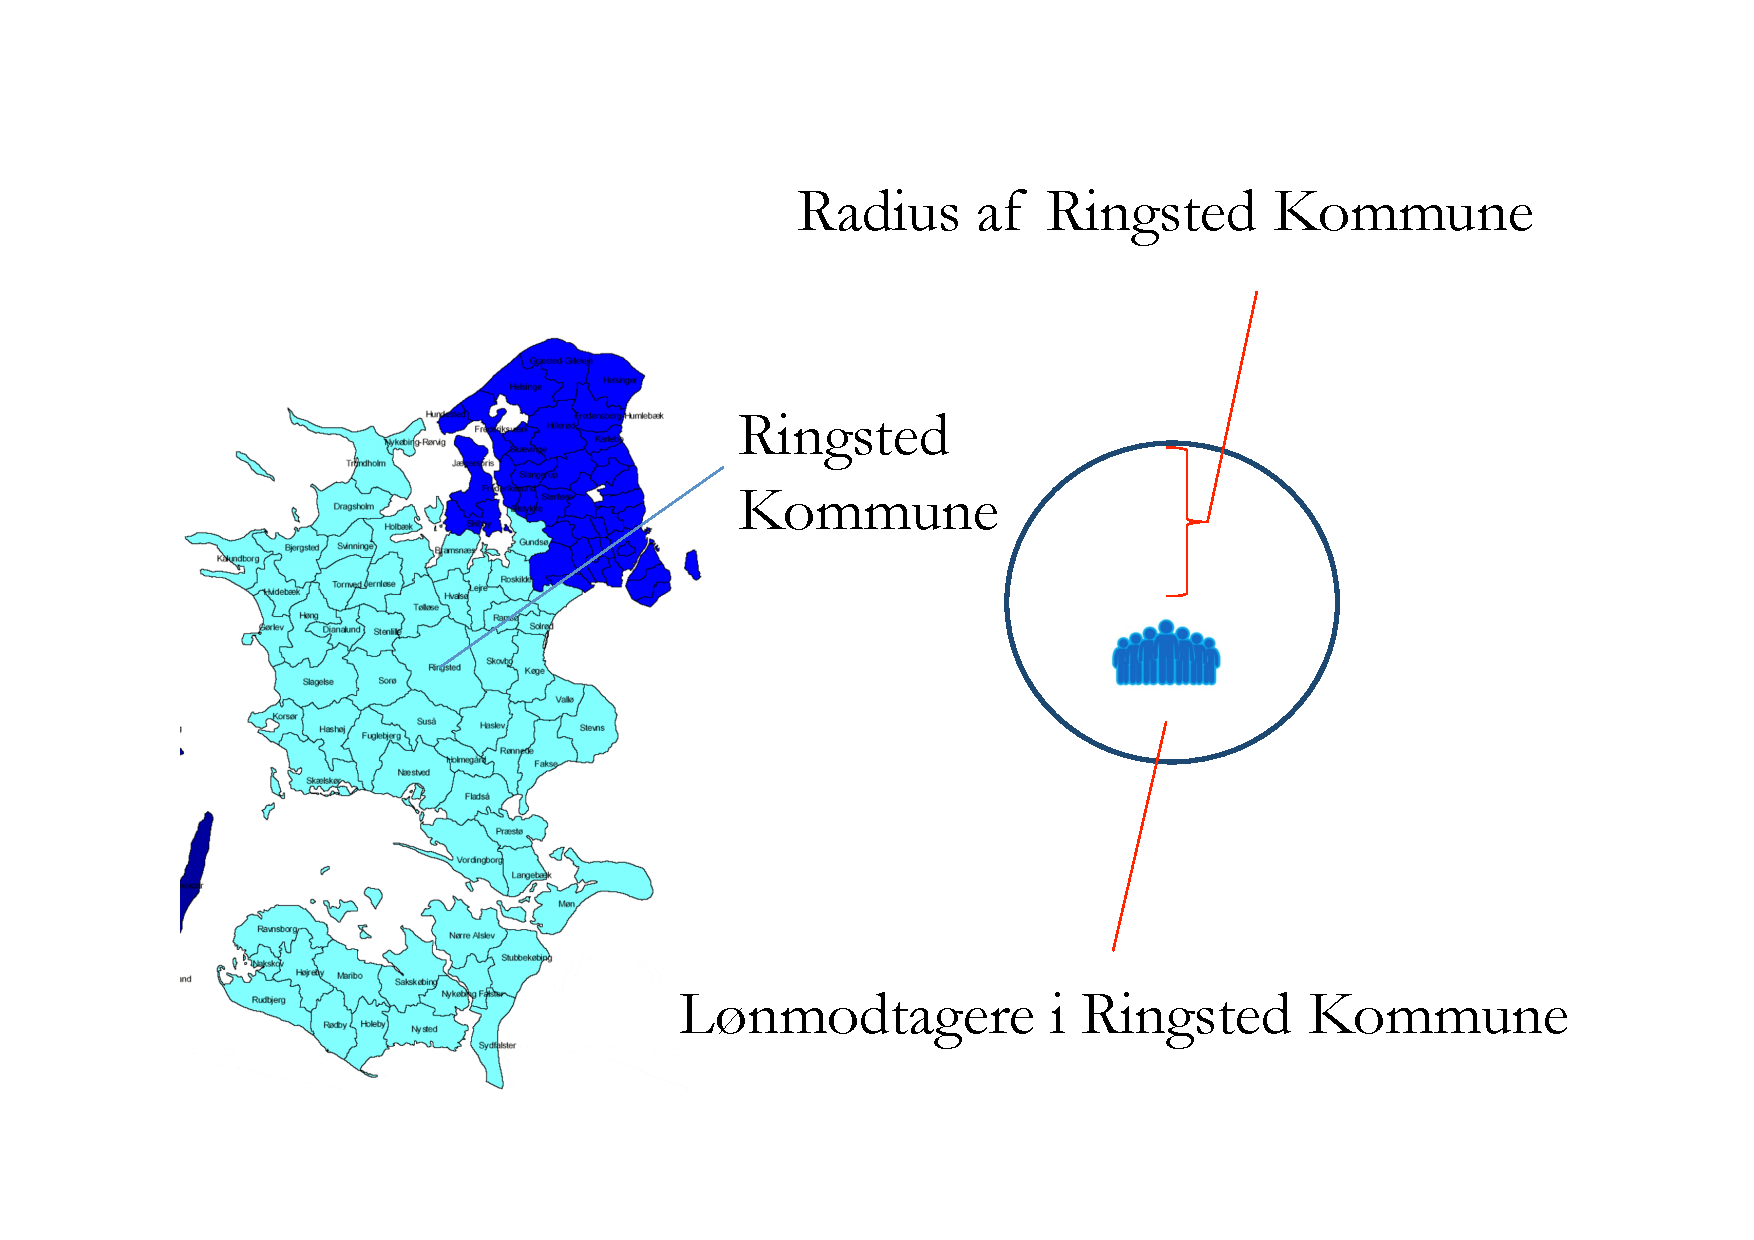
\includegraphics[width=\textwidth]{del1.pdf}
        \caption{Beskæftigelsestætheden}
        \label{fig:del1}
    \end{subfigure}
    \begin{subfigure}[b]{0.49\textwidth}
        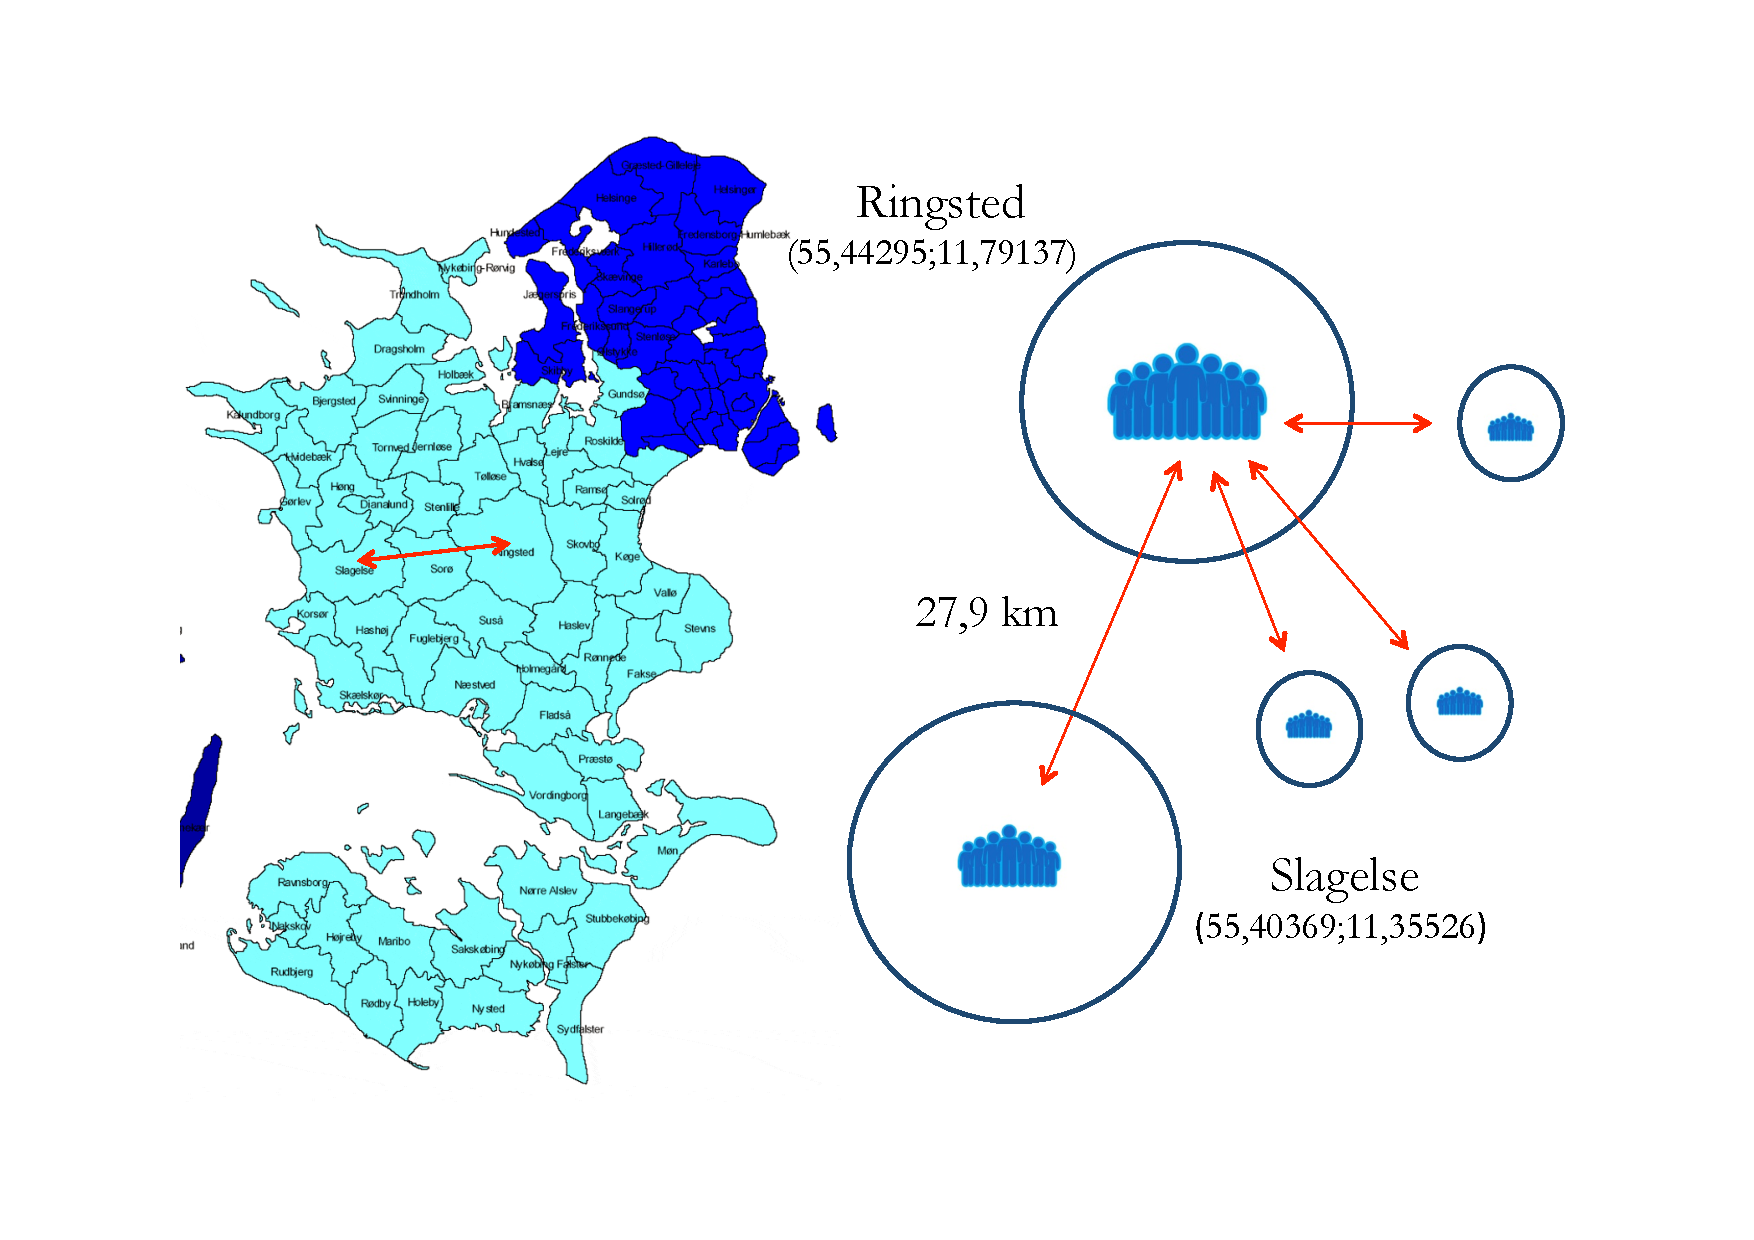
\includegraphics[width=\textwidth]{del2.pdf}
        \caption{Potentielle marked}
        \label{fig:del2}
    \end{subfigure}
  \caption{Caption here}
  \label{fig:metode}
\end{figure}




Til vores analyse har vi valgt, at konstrure parameteren effektiv tæthed, $ED$, i tråd med Grahams metode jf.\cite{graham2007agglomeration}. Fremgangsmetoden kan med fordel forklares med et eksempel som illusteret i figur \ref{fig:metode}. Vi tager de enkelte kommuner, her Ringsted Kommune, og benytter antal af registerbaseret beskæftigelse efter arbejdssted\footnote{Registerbaseret arbejdsstyrke, beskæftigelse, tabel RAS301, Danmarks Statistik} til skalaen af den økonomiske aktivitet. For at udregne tætheden af beskæftigelsen i Ringsted Kommune, finder vi forholdet mellem beskæftigelsen i kommunen og kommunensstørrelse målt på radius kilometer, det betyder at vi implicit antager at kommunerne er cirkelformet. Når vi kender arealet på kommunerne, kan vi blot udregne radius ved hjælp af formlen for radiusen af en cirkel. Denne antagelse viser sig nyttig, når vi skal udregne den relative anstand kommunerne og deres økonomiske aktivitet i mellem. Derefter skal vi bestemmer midtpunkten alle kommunerne, for så at udregne beskæftigelsen per afstandskilometer til alle de 97 andre kommuners midtpunkt. 

$ED$ måler altså den agglomeration som hver virksomhed oplever givet deres placering i Danmark. Første led er selve agglomerationen i hjemkommunenen, $j$, mens andet led er den agglomerationseffekt virksomhederne oplever fra resten af landets kommuner som er faldende i aftand. Virksomhederne i Ringsted Kommune påvirkets altså positivt af en høj beskæftigelse i hjemmekommune, samtidigt påvirkets virksomhederne relativt mere af en høj beskæftigelse i nærliggende kommuner, såsom Slagelse, forhold til jyske kommuner. En væsenligt afgrænsning i vores mål er, at vi ikke tilader agglomerationeffekter på tværs er landegrænser. Det betyder at byer som Flensborg og Malmø ikke indgår i analysen, men pendlerne som rejser på tværs af landene for at arbejde indgår i bæskiftigelsen. Hvis agglomerationseffekter skal indgå i evalueringen af national politik initiativer er tabet ved denne forsimpling ikke stor - hvis derimod fordelen ved en Øresundsbro eller Fermenforbindelse skal evalueres kan analysen med fordel udvides. Den effektive tæthed kan opskrives på følgende vis: 

\begin{equation}
   ED^j_t = \frac{L^j_t}{Radius_j} + \sum_{k=1}^{k \neq j} \frac{L^k_t}{d_{kj}}, \quad Radius_j = \sqrt{\frac{A_j}{\pi}}
 \end{equation} 
 hvor $d_{kj}$ er afstanden mellem kommune $k$ og $j$. 
 

For at finde afstandene mellem alle 98 kommuner i Danmark, benytter vi en såkaldt API. En API gør det muligt at automatisere forspørgelser til en server, i dette tilfælde til servicen Google Maps gennem programmet \textsf{R}. Ved at sende navnet på kommune returnere Google Maps en lokalation i form af koordinat i breddegrader og længdegrader. Vi antager at denne lokation er det approksimative økononomiske midtpunkt af en given kommune. 

Dernæst udregner vi afstanden mellem to kommuners koordinater vha. Haversine-formel\footnote{Skriv en lille historie}. Haversine-formel beregner den korteste afstanden mellem to punkter på en sfære, hvilket netop giver fulgefulgt mellem to kommnuernes midtpunkter. Således kan vi udregne afstandende på kryds og tvær af alle kommuner i en $98\times 98$ symmetrisk matrice. Her er det vigtigt at pointere, at vores afstandsmål ikke tager hensyn til den faktiske kørselsafstand mellem to kommuner. Dette betyder at tolkning af parameteren er den procentvise produktivitetsgevinsten hvis afstanden mellem virksomheder/arbejdskraften mindske med en procent. 

Vi udregner $ED$ for perioden 2008-2015\footnote{En oversigt over effektiv tæthed i perioden 2008-2015 for alle 98 kommuner findes i Appendix}. Hvis vi betragte gennemsnittet af variablen i løbet af perioden, ser vi at de kommuner som er placeret i hovedstadsområdet har den højste værdi. Dette skyldes den høje tæthed af beskæftigelse i København og Frederiksberg. Frederiksberg, Rødovre og København har de tre højste værdi, efterfulgt af de andre kommuner i Storkøbenhavn. Yderligere se vi nogle af de større midtsjællandske kommuner også drager fordel af deres relative afstand til hovedstadsområdet. Aarhus er placeret som nummer 32, efterfulgt af nogle nabokommuner såsom Skanderborg og Odder. Fyns og midtjyllands kommuner findes midt på listen. Den lave ende af listen er kendetegnet ved kommuner, vis placering ofte betegnes som værende i den rådne banan. Det er kommuner som er placeret tæt på den jyske vestkyst. Dette er kommuner såsom Frederikshavn, Hjørring Thisted og Lemvig. I bunden af listen finder vi Bornholm og Læsø som 'staffes' for både at have en tynd besæftigelsestæthed og deres geografiske placering.

Hvis vi betragter ændringen i effektiv tæthed fra 2008 og 2015 tegner der sig en klart billed af urbanisering omkring hovedstaden. Dette er illusret på Danmarkskortet i figur \ref{fig:aendring}. Region Hovedstaden er som en den eneste region, hvor den effektive tæthed har udviklet sig positivt. Aarhus og de omkringliggende kommuner er næsten uændret i perioden, altså neutral eller svag mindskning af effektiv tæthed. De kommuner hvor udviklingen har været mest negativ på tværs af den 'rådne banan', atlså Midt og Vestjylland, Sønderjylland,Fyn og Sydsjælland.

\begin{figure}[tb] 
  \centering
  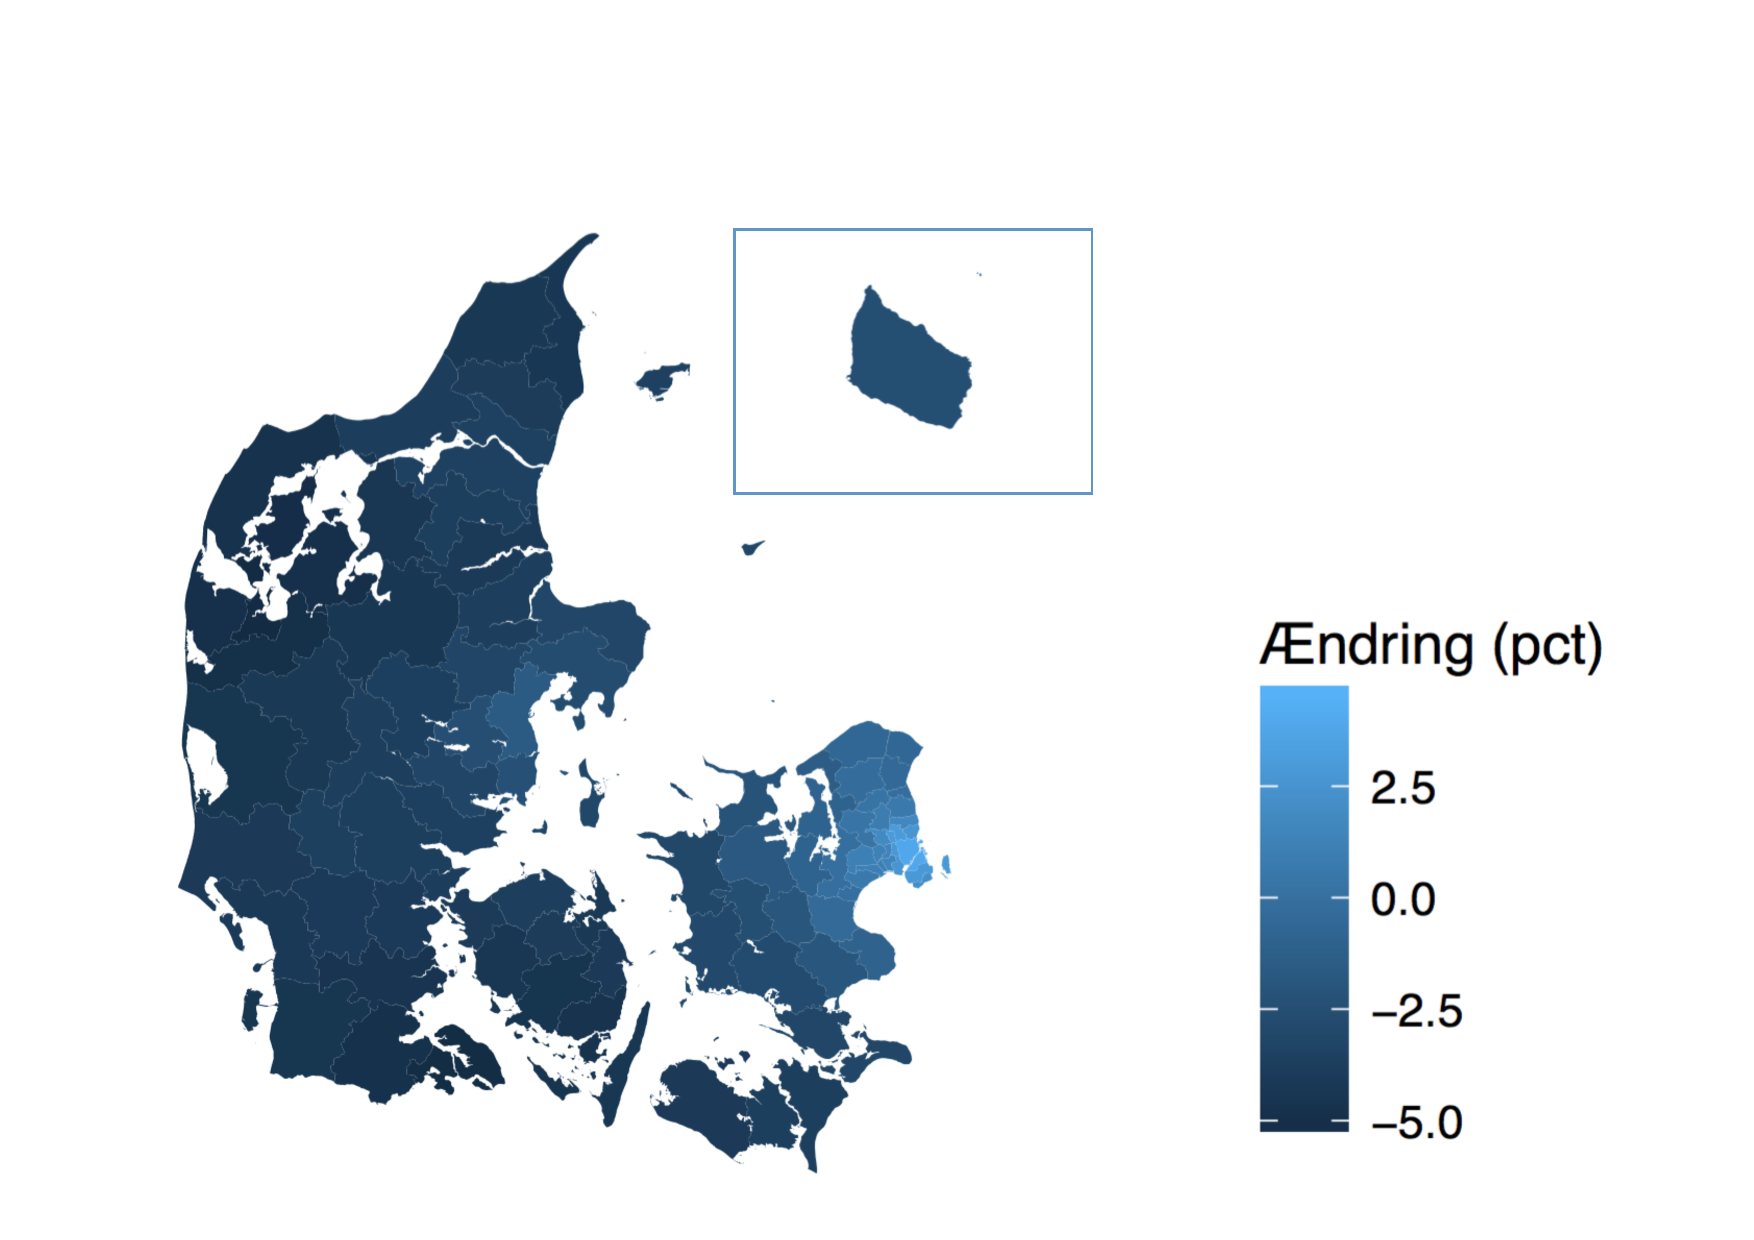
\includegraphics[width=\textwidth]{andring.pdf}
  \caption{Ændring i effektiv tæthed i Danmark 2008-2015, pct.}
  \label{fig:aendring}
\end{figure}

  
  
  %Skrald
  %Opgørelse af dette For at medtage intensiteten på tværs af kommunerne, sætter vi antal beskæftigede i forhold til arealet af kommunerne. Fordelen ved at benytte beskæftigelsestæthed istedet for indbyggertætheden er: 1) antal beskæftigede fanger bedre produktivitetsfordelen ved geografiske konsentreret økonomisk aktivitet, mens at indbygger også vil agere som proxy for urbanisering og eventuelle traffik omkostninger. Ved at benytte tætheden, altså antal eskæftigede lønmodtagere forhold til areal, gør målet robust overfor forskellige kommune størrelser \cite[pp. 335.]{melo2009meta}.
 
%men tager ikke højde for l. Forskellen på lokaliseringsøkonomi og ur
%Graham har estimeret forskellige effekter ved urbanisering vs. clusters i et andet papir (Graham 2006)  
 
 

\section{Metode}
For at kunne måle agglomerationens effekt for danske virksomheder estimerer vi en \emph{agglomerationselasticitet} ved at estimere en produktionsfunktion for virksomheder i private byerhverv. Derved er det muligt at vurdere indenfor hvilke områder agglomeration betyder mest relativt til andre brancher -- og i givet fald hvor meget. På den måde kan vi estimere, hvor meget agglomeration betyder for virksomhedernes værditilvækst, eller med andre ord: Hvor meget af den generede værditilvækst i danske virksomheder skyldes arbejdskraften efficiente densitet?
\section{Estimation af produktionsfunktionen}
For at kunne svare på dette har vi estimeret en produktionsfunktion for virksomhederne -- fordelt efter forskellige branchegrupperinger. Følgende afsnit forklarer metoden, vi har valgt til at bestemme effekten af agglomeration.

Vi antager, at virksomhedernes produktion følger en Cobb-Douglas funktion. 
\begin{equation}
	Y_{it} = A_t K_{it}^{\beta_k} L_{it}^{\beta_l} 
	ED_{it}^{\beta_{ed}}  
\end{equation}
$ED_{it}$ er arbejdskraftens \emph{efficiente densitet}, der for den enkelte virksomhed indgår som en eksternalitet.
Transformeret til logaritmisk form er virksomhedens produktion derfor givet ved følgende relation:
\begin{equation}
	y_{it} = \alpha_t + \beta_l l_{it} + \beta_{ed} ed_{it} + \beta_{k} k_{it} + \epsilon_{it}
	\label{eq:prodfunk_ED_01}
\end{equation}
hvor $y$ er virksomhedens værditilvækst, $l_{it}$ er virksomhedens input af arbejdskraft og $k_{it}$ er virksomhedens input af kapital. Målet er således at estimere $\beta_{ed}$, der er vores agglomerationselasticitet.

\textbf{Hvis vi estimerede (\ref{eq:prodfunk_ED_01}) ved hjælp af OLS, skulle vi for at få et konsistent resultat kræve, at virksomhedernes brug af fx arbejdskraft skulle være uafhængigt af hinanden}. Men da vi må formode, at virksomheder med høj produktivitet anvender mere arbejdskraft og kapital end andre, siger vi derfor, at modellen udtrykt ved (\ref{eq:prodfunk_ED_01}) har et endogenitetsproblem.

Litteraturen fremstiller flere metoder til at korrigere for dette; vi har valgt at følge Levihnson og Petrins metode \cite{levinsohn2003estimating}, der benytter virksomhedernes forbrug af mellemvarer i produktionen til at kontrollere for endogenitetsproblemet. I vores model er metoden udvidet med en parameter for agglomerationen, nemlig $\beta_{ed} ed_{it}$.

Levihnson og Petrins metode foregår i to trin \cite[p. 115ff.]{petrin2004production}. Første trin består i af finde et konsistent estimat for de frie variable i modellen, her $\beta_l$ og $\beta_{ED}$. Modellen er følgende\footnote{Fodtegnet $i$ er udeladt af hensyn til overskuelighed, selvom estimationen foretages på paneldata.}.
%%%%%%%%%%%%%%%%%
\begin{equation}
	y_{t} = \beta_0 + \beta_l l_t+ \beta_{ed} ed_t +
	\beta_k k_t + \beta_t m_t + \omega_t + \eta_t
	\label{LP_01}
\end{equation}
%**********************************************
hvor $m_t$ er virksomhedernes forbrug af mellemvarer. Modellens residualer deles på i to dele, $\omega_t + \eta_t$. $\eta_t$ angiver den del af residualet, der er uafhægigt af kapital, mens $\omega_t$ er den del af residualet, der skaber det ovennævnte endogenitetsproblem. Det betyder, at metodens grundlæggende formål er, at korrigere for det bias, der opstår gennem den endogene del af residualet, 
$\omega_t$.

Levihnson og Petrin foreslår brug af mellemvarer som proxyvariabel for det ukontrollerede produktivitetsshock i $\omega_t$. Intuitionen bag dette resultat er, at for enhver given mængde af kapital i virksomheden, vil virksomheder med høj produktivitet skrue op for produktionen -- og dermed også for mellemvareforbruget, fx energi. Denne mellemregning er en måde at korrigere for effekten af $\omega_t$ på kapital, hvis vi kan påvise en markant positiv sammenhæng mellem $\omega_t$ og virksomhedernes forbrug af mellemvarer.

Levinsohn og Petrin antager, at $m_t$ er en funktion af kapital og $\omega_t$, $m_t = m(k_t , \omega_t)$, og viser, at denne funktion under visse betingelser er monotont stigende i $\omega_t$ \cite[322-323]{levinsohn2003estimating}. Når dette er tilfældet, kan funktionen inverteres, og det uobserverede led $\omega_t$ kan udtrykkes som en funktion af to observerede størrelse, kapital og mellemvarer.
\begin{equation}
	\omega_t = \omega(k_t , m_t)
	\label{eq:InverseOmega}
\end{equation}

\begin{align}
	y_t &= \beta_l l_t + \beta_{ed} ED_t + \phi ( k_t , m_t)
	\label{eq:LPProdFunkt02}\\
	\phi ( k_t , m_t) &\equiv \beta_0 + \beta_k + \omega (k_t , m_t) \notag
\end{align}
Som approksimering af $\omega ( k_t , m_t)$ benytter Levinsohn og Petrin sig af et 3. grads polynomium interaktionsled mellem kapital og mellemvarer. Det indsættes i (\ref{eq:LPProdFunkt02}), hvormed $\beta_l$ og $\beta_{ed}$ kan estimeres nonlineært.
\begin{align}
	y_t &= \beta_l l_t + \beta_{ed} ED_t + \delta_0 + \sum_{i=0}^{3} \sum_{j=0}^{3-i} d_{ij} k_t^i m_t^j 
	\label{eq:LPSaturatedProdFunction}
\end{align}
Ved estimering af (\ref{eq:LPSaturatedProdFunction}) ved brug af OLS har vi estimatorer for $\beta_l$ og $\beta_{ed}$, der er konsistente. Bemærk at $\delta_0 \neq \beta_0$ da den sidste gemmer sig i interaktionen i 3. gradspolynomiet i (\ref{eq:LPSaturatedProdFunction}). Dette afslutter det første trin.

\textbf{Formålet med det andet trin er at finde et konsistent estimat for $\beta_k$.} 
Ved at benytte $\beta_l$ og $\beta_{ed}$ fra estimering af (\ref{eq:LPSaturatedProdFunction}), kan vi finde et estimat for $\hat{\phi}$ på følgende måde
\begin{align}
	\hat{\phi} &= \hat{v_t} - \hat{\beta_l} l_t - \hat{\beta_{ed}} ed_t \\
	&= \hat{\delta_0} + \sum_{i=0}^{3} \sum_{j=0}^{3-i} \hat{d_{ij}} k_t^i m_t^j - \hat{\beta_l} l_t - \hat{\beta_{ed}} ed_t 
	\label{eq:LPfindenPhi}
\end{align}
Fra (\ref{eq:LPfindenPhi}) kan vi dermed finde et estimat for $\omega_t$:
\begin{equation}
	\hat{\omega} = \hat{\phi} - \beta^*_k k_t
	\label{eq:LPFindenOmega}
\end{equation}
hvor $\beta_k^*$ er et initialt gæt for $\beta_k$. Ifølge Levihnson og Petrin kan det antages, at $\omega_t$ følger en markov proces, som de nonlinenært estimere ved hjælp af et 3. grads polynomium.
\begin{equation}
 	\hat{E[w_t | w_{t-1}]} = \gamma_0 + \gamma_1 \omega_{t-1} + \gamma_2 \omega^2_{t-1} + \gamma_3 \omega^3_{t-1} + \epsilon_t
 	\label{eq:markovOmega}
 \end{equation} 
Et estimat for $\beta_k$ findes nu gennem en golden section optimerings rutine på følgende kvadrat ved at minimere følgende kvadrat:
\begin{equation}
	\min_{\beta^*_k} 
	\left( 
		v_t - \hat{\beta_l} l_t - \hat{\beta_{ed}} ed_t 
		- \beta^*_k k_t - \hat{E[w_t | w_{t-1}]} 
	\right)^2
	\label{eq:LPOptimization}
\end{equation}
$\hat{\beta_k}$ estimeres iterativt igennem (\ref{eq:LPFindenOmega}) og (\ref{eq:markovOmega}), der bidrager til (\ref{eq:LPOptimization}). Standardafvigelser og varians-kovariansmatricen benyttet til Wald-test for konstant skalaafkast findes bed hjælp af bootstrapping.

\paragraph{Bootstrapping}
Da (\ref{eq:LPOptimization}) skaber et estimat af $\hat{\beta_k}$ på baggrund af en kompliceret optimerings procedure, er det derfor ikke muligt at udregne analytiske værdier for standardafvigelserne. Derfor benytter Levinsohn og Petrin sig af bootstrapping, der er en såkaldt \emph{resampling} metode.

Bootstrapping udregner parameterestimaterne for modellen ud fra en stikprøve med tilbagelægning på samme størrelse som datasættet. Når dette gøres tilpas mange gange, kan standardafvigelserne for de disse estimater, der laves på baggrund af de gentagne stikprøver, benyttes som konsistente standardafvigelser for vores variable i modellen.

Da vores model er kompliceret og i nogen grad komputeringstung har vi valgt at benyttes 50 iterationer til at konstruere standardafvigelserne præsenteret i tabel ???.
\subsection{Input til produktionsfunktionen}
\textbf{Input til $l_t$ er Kvalitetskorrigeret arbejdskraft}
Når virksomhedernes anvendelse af arbejdskraft indgår i produktionen, er det i et produktivitetsøjemed vigtigt at tage højde for, at medarbejderens produkvitet afhænger af især uddannelse og erfaring.

Derfor har vi et kvalitetskorrigeret arbejdsindeks som arbejdsinput i produktionsfunktionen \cite[s. 5]{dors2010baggrund}. Denne tager højde for, hvor meget den enkelte virksomhed inddrager af arbejdskraft, så der tages højde for medarbejderens uddannelse og erfaring. Uddannelsesniveau og erfaring kombineres i Danmark Statistiks registre med indberettede regnskabsdata så der for den enkelte virksomhed kan skabes et kvalitetskorrigeret arbejdsinput.

Kvalitet følger DØRS definition og udregnes som \cite[s. 5]{dors2010baggrund}:
\begin{equation}
	\bar{L_{it}} = 
	L_{i0t} + \sum_{f=1}^{F-1} \frac{\bar{w}_{fgt}}{\bar{w}_{0gt}} 
	L_{ift}
\end{equation}
$f$ er her en gruppering af beskæftigelsen efter kvalitet. Fx er $f=0$ en ufaglært medarbejder med lav erfaring, $f=1$ er en ufaglært medarbejder med 5-10 års erfaring osv. CHECK!!!!!!
$L_{ift}$ er så antallet af årsværk i virksomheder med kvalitet $f$. Dermed er det muligt at korrigere for kvaliteten af arbejdskraften, så en times præsteret nu tæller forskelligt alt efter produktivteten.

I produktionsfunktionen fra (\ref{eq:LPProdFunkt02}) indgår den kvalitetskorrigerede arbejdskraft som $l_{it} = \log(L_{it})$.  

\section{Beskrivelse af data}
Vi har benyttet Danmarks Statistiks virksomhedsregister som baggrund for estimeringen. Data tilgængeligt for os er i årene 2008 -- 2013, hvori vi har 45.751 observationer fordelt på ca. 17.000 cvr numre. Datasættet er ikke et fuldt panel. For en beskrivelse af agglomerationsvariablen, jf. kapital ???.

Virksomhederne er kun indenfor branche i private byerhverv, hvilket vil sige branchegrupperne Industri, Bygge og anlæg, Transport, Hoteller og restauranter, Handel, Information og Kommunikation, Videnservice og Operationel service.

Der er lavet visse restrektioner på registrene. Blandt andet er virksomheder med færre end fem ansatte. 

\paragraph{Kapitalapparat} 
Kapitalinput er virksomhedernes materielle og immatrielle aktiver fra regnskabsstatistikken, hvorefter den deflateres. Denne deflatering sker ved hjælp af deflateren for kapital fra Danmarks Statistiks nationalregnskab for de relevante år\footnote{Fordelt på branche??}.

\begin{itemize}
	\item Spørg Lill om metoden
\end{itemize}

\paragraph{Antagelser for konsistent estimering af ed}
%%Det jeg vil skrive nu
% - Bootstrapping
% - Bootstrapping
\section{Resultater}
I dette afsnit præsenterer vi de estimerede resultater henholdvist for industri og private service samlet, og opdelt på underbrancher. Vi estimere ligeldes agglomerationseffekter samlet for alle brancher, hjemmemarked og udlandskonkurrende. 


Industri 
Teknik 

Den første tabel, tabel \textbf{INDSÆT ref)} viser resultaterne for estimation af produktionsfunktionerne for industrierhverv. Indledningsvist kan vi se at der findes en relativ stor spredning af antal observationer fordelt på de forskellige underindustrier. I medicinalindustri, tekstil- og læderindustri og transportmiddelindustri finder vi industrierne med færrest observation, mens metalindustri, maskinindustri og føde-, drikke- og tobaksvareindustri er de største. Modellen medfører $R^2$ fra 0,33 til 0,92, dog med en relativt høj $R^2$ som forklarer mere end 50\% af variationen for største delen af industrierne. 

Skriv om $\beta_L$
Skriv om RTS


Hvis vi nu betragter estimaterne for agglomerationselasticiteten i produktionen for industrierhverv, hvilken givet ved $\beta_{ed}$, ser vi at 9 ud af de 12 industrierhvervene ingen signifikant agglomerationseffekt har. Det vil altså sige, at vi ikke kan afvise nul-hypotsesen; at agglomeration ingen effekt har på produktionen i industrien. Vender vi os mod teorien og tidligere studier, som beskrevet tidligere, så forventer vi at denne type virksomheder typisk vil placere sig væk fra urbaneområder, dels fordi dette kan holde omkostningerne nede på inputfaktorerne, hord, bygninger, leje og arbejdskraft er typisk billigere i disse områder. Og dels på grund af tilgangen til god infrastruktur således at råmatriale og færdigvare let kan komme til og fra virksomhederne.      

Vi finder en positiv og signifikant agglomerationselasticitet de resterende 3 industribrancher, navnligt føde-, drikke- og tobaksvareindustri, maskinindustri og Møbel og anden industri mv. 

Føde-, drikke- og tobaksvareindustri drager nytte af at placere produktionen i områder med høj effektiv tæthed. 

Møbel og anden industri mv dækker over møbelfremstilling, legetøj og anden fremstillingsvirksomhed og reperation og intallation af maskiner og udstyr. Argumenterne fra fødevareindustri giver samme intuitive mening for fremstilling af møbler og legetøj. Reperation og installation 


Intuitionen for insiginikante resultater

s

Vender vi os mod privat serivce er billedet anderledes. Her har vi mange observationer per underbranche, eksempelvis har vi i den største branche handel (G) flere observationer end hele industrien - den næststørste branche er bygge og anlæg. Færrest observationer finder vi i hotel og resturanter og rejsebureauer, rengøring og anden operationel service. Modellens $R^2$ spænder fra 0.55 til 0.77, altså generelt højere end i industribrancherne. 


Skriv om $\beta_L$
Skriv om RTS


Vi finder positiv og siginifikante agglomerationselasticiteter i alle brancher i privat service. I rejsebureauer, rengøring og anden operationel service finder vi den lavest elasticitet, 8\%, mens at den er godt tre gange så stor i videnservice. 




\begin{table}[tb]
\centering
\caption{My caption}
\label{my-label}
\begin{tabular}{@{}lrrrrrrr@{}}\arrayrulecolor{MidnightBlue}\toprule
v             & C, samlet & CA       & CB       & CC       & CE       & CF      & CG       \\ \arrayrulecolor{MidnightBlue}\midrule
$\beta_l$      & 0.695***  & 0.621*** & 0.715*** & 0.748*** & 0.704*** & 0.462** & 0.676*** \\
              & (0.013)   & (0.039)  & (0.074)  & (0.039)  & (0.071)  & (0.190) & (0.039)  \\
$\beta_k$      & 0.117***  & 0.116*   & -0.019   & 0.118**  & 0.202    & 0.271   & 0.305**  \\
              & (0.024)   & (0.066)  & (0.168)  & (0.049)  & (0.192)  & (0.218) & (0.121)  \\
$\beta_{ed}$ & 0.051***  & 0.111*** & -0.004   & 0.049    & 0.084    & 0.084   & 0.024    \\
              & (0.015)   & (0.040)  & (0.121)  & (0.033)  & (0.075)  & (0.175) & (0.045)  \\
              &           &          &          &          &          &         &          \\
\emph{N}  & 9.959     & 1.274    & 246      & 963      & 280      & 106     & 1.100    \\
$\beta_0$         & 0.460     & 0.903    & 1.933    & -0.303   & -0.783   & 1.705   & -0.952   \\
$R^2$            & 0.606     & 0.502    & 0.362    & 0.696    & 0.757    & 0.566   & 0.920    \\
RTS$_1$          & 0.863     & 0.849    & 0.692    & 0.915    & 0.990    & 0.817   & 1.005    \\
RTS$_2$           & 0.812     & 0.738    & 0.696    & 0.867    & 0.906    & 0.733   & 0.981    \\
Wald$_1$         & 17.880    & 3.740    & 1.634    & 1.197    & 0.003    & 0.589   & 0.001    \\
Wald$_2$         & 44.480    & 14.700   & 2.429    & 4.144    & 0.237    & 1.244   & 0.024   \\ \arrayrulecolor{MidnightBlue}\midrule
\multicolumn{8}{l}{Standardfejl i parantes. Kilde: Danmarks Statistik og egne beregninger.} \\
\arrayrulecolor{MidnightBlue}\bottomrule
\end{tabular}
\end{table}
\begin{table}[tb]
	\centering
	\caption{Output}
	\label{tab:Output2}
	\begin{tabular}{@{}lrrrrrr@{}}
		\toprule
		v            & CH       & CI       & CJ       & CK       & CL       & CM       \\ \midrule
		$\beta_l$    & 0.650*** & 0.848*** & 0.734*** & 0.708*** & 0.635*** & 0.796*** \\
		& (0.035)  & (0.070)  & (0.060)  & (0.032)  & (0.060)  & (0.034)  \\
		$\beta_k$    & 0.105**  & 0.142*   & -0.081   & 0.129*** & 0.044    & 0.112    \\
		& (0.041)  & (0.079)  & (0.117)  & (0.039)  & (0.114)  & (0.085)  \\
		$\beta_{ed}$ & -0.017   & 0.011    & 0.0306   & 0.060**  & -0.046   & 0.090**  \\
		& (0.034)  & (0.080)  & (0.078)  & (0.026)  & (0.163)  & (0.044)  \\
		&          &          &          &          &          &          \\
		\emph{N} & 1.919    & 545      & 418      & 1.783    & 286      & 1.039    \\
		$\beta_0$    & 1.732    & -1.170   & 2.077    & 0.010    & 2.825    & -1.123   \\
		$R^2$        & 0.580    & 0.775    & 0.326    & 0.674    & 0.492    & 0.700    \\
		RTS$_1$      & 0.737    & 1.001    & 0.683    & 0.897    & 0.634    & 0.998    \\
		RTS$_2$      & 0.755    & 0.990    & 0.653    & 0.837    & 0.680    & 0.907    \\
		Wald$_1$     & 18.580   & 4.28e-05 & 5.194    & 3.880    & 2.478    & 0.001    \\
		Wald$_2$     & 22.390   & 0.010    & 8.558    & 14.630   & 5.955    & 1.318   
		\\ \midrule
		\multicolumn{7}{l}{Standardfejl i parantes. Kilde: Danmarks Statistik og egne beregninger.} \\
		\bottomrule
	\end{tabular}
\end{table}
\begin{table}[tb]
	\centering
	\caption{Ouput}
	\label{tab:ouput3}
\scalebox{0.8}{
	\begin{tabular}{@{}lrrrrrrrr@{}}
		\toprule
		v            & Privat Service, samlet & F        & G        & H        & I        & J        & N        & M        \\ \midrule
		$\beta_l$    & 0.825***               & 0.724*** & 0.893*** & 0.721*** & 0.714*** & 0.788*** & 0.721*** & 0.825*** \\
		& (0.009)                & (0.017)  & (0.013)  & (0.037)  & (0.033)  & (0.0341) & (0.028)  & (0.030)  \\
		$\beta_k$    & 0.055***               & 0.091*** & 0.055*** & 0.144*** & 0.060**  & 0.0826** & 0.072*** & 0.051*** \\
		& (0.006)                & (0.024)  & (0.015)  & (0.039)  & (0.025)  & (0.0337) & (0.027)  & (0.018)  \\
		$\beta_{ed}$ & 0.187***               & 0.107*** & 0.137*** & 0.124*** & 0.147*** & 0.185*** & 0.079*** & 0.221*** \\
		& (0.006)                & (0.014)  & (0.017)  & (0.029)  & (0.025)  & (0.0246) & (0.024)  & (0.021)  \\
		&                        &          &          &          &          &          &          &          \\
		\emph{N}   & 32.792                 & 5.290    & 14.022   & 2.776    & 1.678    & 2.625    & 2.487    & 3.914    \\
		$\beta_0$    & -2.022                 & -0.448   & -2.295   & -0.946   & -0.561   & -1626    & 0.514    & -2.272   \\
		$R^2$        & 0.716                  & 0.651    & 0.783    & 0.695    & 0.550    & 0.774    & 0.652    & 0.727    \\
		RTS$_1$      & 1.067                  & 0.922    & 1.084    & 0.989    & 0.921    & 1055     & 0.872    & 1.097    \\
		RTS$_2$      & 0.880                  & 0.815    & 0.947    & 0.864    & 0.775    & 0.870    & 0.793    & 0.877    \\
		Wald$_1$     & 38.640                 & 8.353    & 17.630   & 0.0484   & 2.451    & 1500     & 10.380   & 6.489    \\
		Wald$_2$     & 149.900                & 41.530   & 11.170   & 8.616    & 30.620   & 8365     & 29.910   & 20.220  \\
		\midrule
		\multicolumn{9}{l}{Standardfejl i parantes. Kilde: Danmarks Statistik og egne beregninger.} \\
		\bottomrule
	\end{tabular}%
}
\end{table}

\begin{table}[tb]
\centering
\caption{Output}
\label{tab:OutputAlleUdeHjemme}
\begin{tabular}{@{}lrrr@{}}
\arrayrulecolor{MidnightBlue}\toprule
             & Alle brancher & Hjemmemarked & Udland   \\
             \arrayrulecolor{MidnightBlue}\midrule
$\beta_l$    & 0.810***      & 0.832***     & 0.681*** \\
             & (0.007)       & (0.008)      & (0.016)  \\
$\beta_k$    & 0.0663***     & 0.052***     & 0.133*** \\
             & (0.007)       & (0.005)      & (0.020)  \\
$\beta_{ed}$ & 0.169***      & 0.186***     & 0.069*** \\
             & (0.006)       & (0.007)      & (0.012)  \\
             &               &              &          \\
\emph{N}   & 42.751        & 32.530       & 10.221   \\
$\beta_0$    & -1.726        & -2.068       & 0.297    \\
$R^2$        & 0.702         & 0.726        & 0.612    \\
RTS$_1$      & 1.045         & 1.069        & 0.883    \\
RTS$_2$      & 0.877         & 0.884        & 0.814    \\
Wald$_1$     & 20.120        & 51.700       & 19.560   \\
Wald$_2$     & 254.300       & 179.400      & 65.270  \\
\arrayrulecolor{MidnightBlue}\midrule
\multicolumn{4}{p{7cm}}{\raggedright Standardfejl i parantes. Kilde: Danmarks Statistik og egne beregninger.} \\
\arrayrulecolor{MidnightBlue}\bottomrule 
\end{tabular}
\end{table}
%%****************** muligvis skrald
\section{Estimation}
Vi ønsker at estimere følgende output dataset
\begin{equation}
	\ln Y_{it}^{pj} = \alpha^p_0 + \ln K_{it} + \ln L_{it} + ED^j_{t} + \omega^p_{t}
\end{equation}
hvor $i$ er virksomhedsindeks, $p$ kommuneindeks, $t$ angiver tidspunkt i år og $j$ angiver kommune. 

%%%*******************************
\section{Praktisk case/vinkel policy anbefaling}
On the other hand, we denounce with righteousd indignation and dislike men who are so beguiled and demoralized by the charms of pleasure of the moment, so blinded by desire, that they cannot foresee the pain and trouble that are bound to ensue; and equal blame belongs to those who fail in their duty through weakness of will, which is the same as saying through shrinking from toil and pain. These cases are perfectly simple and easy to distinguish. In a free hour, when our power of choice is untrammelled and when nothing prevents our being able to do what we like best, every pleasure is to be welcomed and every pain avoided. But in certain circumstances and owing to the claims of duty or the obligations of business it will frequently occur that pleasures have to be repudiated and annoyances accepted. The wise man therefore always holds in these matters to this principle of selection: he rejects pleasures to secure other greater pleasures, or else he endures pains to avoid worse pains. "On the other hand, we denounce with righteous indignation and dislike men who are so beguiled and demoralized by the charms of pleasure of the moment, so blinded by desire, that they cannot foresee the pain and trouble that are bound to ensue; and equal blame belongs to those who fail in their duty through weakness of will, which is the same as saying through shrinking from toil and pain. These cases are perfectly simple and easy to distinguish. In a free hour, when our power of choice is untrammelled and when nothing prevents our being able to do what we like best, every pleasure is to be welcomed and every pain avoided. But in certain circumstances and owing to the claims of duty or the obligations of business it will frequently occur that pleasures have to be repudiated and annoyances accepted. The wise man therefore always holds in these matters to this principle of selection: he rejects pleasures to secure other greater pleasures, or else he endures pains to avoid worse pains.
\section{Diskussion}
Forslag: Kvalitetsjustering af beskæftigelsen i ED og lag værdier af ED 
\section{Konklusion}
On the other hand, we denounce with righteous indignation and dislike men who are so beguiled and demoralized by the charms of pleasure of the moment, so blinded by desire, that they cannot foresee the pain and trouble that are bound to ensue; and equal blame belongs to those who fail in their duty through weakness of will, which is the same as saying through shrinking from toil and pain. These cases are perfectly simple and easy to distinguish. In a free hour, when our power of choice is untrammelled and when nothing prevents our being able to do what we like best, every pleasure is to be welcomed and every pain avoided. But in certain circumstances and owing to the claims of duty or the obligations of business it will frequently occur that pleasures have to be repudiated and annoyances accepted. The wise man therefore always holds in these matters to this principle of selection: he rejects pleasures to secure other greater pleasures, or else he endures pains to avoid worse pains. "On the other hand, we denounce with righteous indignation and dislike men who are so beguiled and demoralized by the charms of pleasure of the moment, so blinded by desire, that they cannot foresee the pain and trouble that are bound to ensue; and equal blame belongs to those who fail in their duty through weakness of will, which is the same as saying through shrinking from toil and pain. These cases are perfectly simple and easy to distinguish. In a free hour, when our power of choice is untrammelled and when nothing prevents our being able to do what we like best, every pleasure is to be welcomed and every pain avoided. But in certain circumstances and owing to the claims of duty or the obligations of business it will frequently occur that pleasures have to be repudiated and annoyances accepted. The wise man therefore always holds in these matters to this principle of selection: he rejects pleasures to secure other greater pleasures, or else he endures pains to avoid worse pains."



\paragraph{Kvalitetsjusteret arbejdskraft}



\paragraph{Levihnson og Petrin}
Hvad nu hvis jeg skriver noge

Syntaksen for at citere er \cite[pp. 211ff.]{melo2009meta}. 

 % paragraph levihnson_og_petring (end)



\bibliography{prodBib.bib}
\bibliographystyle{plain}
\end{document}